%!TEX root = ../thesis.tex
%*******************************************************************************
%*********************************** Third Chapter *****************************
%*******************************************************************************

\chapter{Bioelectrical impedance plethysmography}  %Title of the First Chapter
\label{chapter impedance}

\ifpdf
    \graphicspath{{Chapter3/Figs/Raster/}{Chapter3/Figs/PDF/}{Chapter3/Figs/}}
\else
    \graphicspath{{Chapter3/Figs/Vector/}{Chapter3/Figs/}}
\fi

Before describing how impedance plethysmography operates, it is better to understand how the principle of bioelectrical impedance is defined. First of all, the term electrical impedance spectroscopy (EIS) is referred as the study of the absorption of energy depending upon the frequency of electromagnetic (EM) waves. When measurements are performed in a biological sample, then this method could be referred either as electrical impedance or bioelectrical impedance~\cite{ivorra2003bioimpedance}. The term to be used in this document will be bioelectrical electrical impedance. The EM spectrum is quite broad, and the interaction with tissue occurs in the frequency range from \SIrange[scientific-notation = engineering]{100}{10000000}{\hertz}~\cite{bertemes2002tissue}. In this thesis, the frequencies of interest are focused in the low-frequency range. Indeed, plethysmography devices operate commonly in the bandwidth below few \si{\kilo\hertz}.

The human body is constituted by four basic tissues known as epithelium which covers and protects the whole surface of the body, muscle which is in charge of the movement, connective tissue that supports and protect organs, and nervous tissue which provides the internal transmission line for the electrical impulses coming from the brain. Cells that constitute these tissues play a fundamental role in terms of current conduction when an analogue current (AC) is applied to the body~\cite{lvovich2012impedance}. Hence, impedance readings vary according to the parameters of these cells as well as its protein content. It is especially significant to understand the geometry and characteristics of the blood cells, which transport $0_2$ around the body. The functionality of these cells and amount per \si{\micro\litre} of human blood were described by table \ref{table:cell} in section \ref{section literature 1}.

As can be noticed from that table, RBC's statistically are more numerous than the other cells and it has particular resistive properties. Its disk shape can be ideally represented as a spherical particle with membranes around the surface, as represented by Figure \ref{fig:cell}. Live cells can be represented as multilayer cells where its internal cytoplasm has a characteristic permittivity ($\epsilon_{cp}$) and conductivity ($\rho_{cp}$). Likewise, these characteristics are similar to the one surrounding the cell called extracellular fluid ($\epsilon_m$ and $\rho_m$). However, the membrane has a very low permittivity ($\epsilon_{MBR}$) and conductivity ($\rho_{MBR}$) behaving as a dielectric. In contrast in dead cells the membrane becomes loose and does not provide resistance to electric current~\cite{lvovich2012impedance}.

\begin{figure}[!htpb]
	\centering
	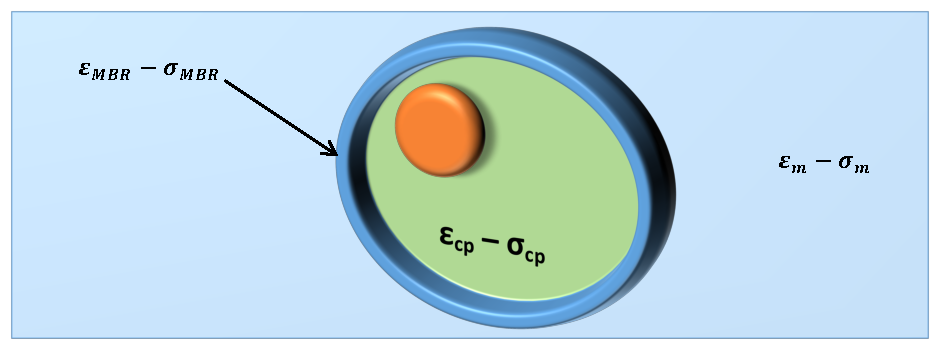
\includegraphics[width=0.8\textwidth,keepaspectratio, trim={0cm 0cm 0cm 0cm},clip]{figure1}    
	\caption[Cell permeability and conductivity distribution]{Representation of a cell with its electric characteristics. Internal cytoplasm characteristic permittivity $\epsilon_{cp}$ and conductivity $\rho_{cp}$. Extracellular fluid permittivity $\epsilon_m$ and conductivity $\rho_m$). Membrane permittivity described as ($\epsilon_{MBR}$) and conductivity ($\rho_{MBR}$).}
	\label{fig:cell}
\end{figure}

A cell can change its internal cytoplasm by two different means either changing the permeability of their bilayer lipid membrane (BLM) or by using ionic channels or pumps. The BLM is about \SI{7}{\nano\meter} thick, by altering its permeability it allows lipids and water molecules to pass through~\cite{ivorra2003bioimpedance}. The interface extracellular-membrane-intracellular ($\rho_m \rightarrow \rho_{MBR} \leftarrow \rho_{cp}$) behaves as a capacitor because the membrane is a dielectric between two conductors, which is represented as $C_m$ in figure \ref{fig:cell model}.

On the other hand, parallel to BLM the ionic channels and pumps enhance membrane’s functionality. Ionic channels or “channel proteins” allow transport and exchange of certain types of ions such as $Na^{+}$, $K^{+}$, Chloride ($Cl^{-}$) and Calcium ($Ca^{2+}$) between the inside and outside of the cell~\cite{lvovich2012impedance}. Ion pumps are caused by sensitivity of the membrane to a voltage; it is also responsible for the membrane’s non–linear properties to low voltage. This pump also causes cell polarisation that allows the flow of ion charges in the body. Electrically, these channels act as a resistor ($R_m$).

\begin{figure*}[!htbp]
	\centering
	\begin{subfigure}[t]{0.5\textwidth}
		\centering
		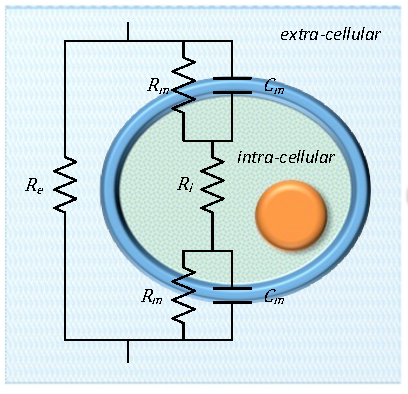
\includegraphics[height=6.5cm]{figure2a}
		\caption{Cell's equivalent circuit model}
		\label{fig:cell model}
	\end{subfigure}%
	~ 
	\begin{subfigure}[t]{0.5\textwidth}
		\centering
		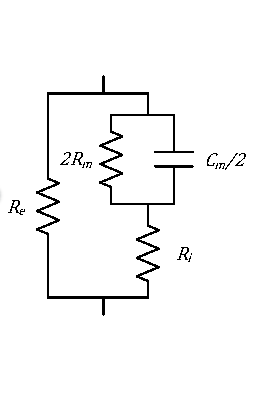
\includegraphics[height=6.5cm]{figure2b}
		\caption{Simplified circuit model}
		\label{fig:cell simp model}
	\end{subfigure}
	\caption[Electrical model of the cell]{Electrical model of the cell and its simplified version. $R_e$ is the resistivity of the extracellular medium, $R_i$ is the resistivity of the intracellular medium and $R_m$ and $C_m$ are the resistivity and capacitance of the membrane.}
	\label{fig:cell models}
\end{figure*}

According to previous analysis, the cell can be simplified in an equivalent electric circuit model as shown in Figure \ref{fig:cell models}. This model shows that if AC is pumped into the extracellular medium, there are two possible paths for the current to go through. One way is around the cell which is represented by the resistive characteristic of the extracellular medium ($R_e$). In the second route, current flows through the cell. Indeed, AC may flow initially either over the BLM which is a represented as a capacitance ($C_m$) or across ionic channels ($R_m$).Once in the cell, current travels via the intracellular medium ($R_i$) that is mostly resistive. Lastly, the electrical current leaves the cell through the membrane, which it is again the same $C_m$ and $R_m$.

Since $C_m$ and $R_m$ have the same values when the current enters and exits the cell, this can be simplified in the electric model as two resistors in series ($2R_m$) and two capacitances in parallel ($C_m/2$) as can be seen in figure \ref{fig:cell simp model}.


When an EM field is applied to the tissue, cells respond according to the frequency applied showing three distinctive areas in the spectrum as described by Schawn et al.~\cite{schwan1957electrical,schwan1962electrical}. Figure \ref{fig:ABG dispersion} displays the dielectric response against frequency, which reveals valuable information about the functional and structural properties of the cell~\cite{lvovich2012impedance}. According to the graph, there are three denominating areas $\alpha$, $\beta$ and $\gamma$ dispersion. Firstly, $\alpha$ dispersion (from \SI{10}{\hertz} to a few \si{\kilo\hertz}) is generally associated with frequency dependent properties of the cells’ membrane. Secondly, $\beta$ dispersion (\SI{10}{\kilo\hertz} to several \si{\mega\hertz}) is related to the dielectric property of the cell membrane and the interaction between the internal and external mediums. Finally, $\gamma$ dispersion (> \SI{10}{\giga\hertz}) is due to dielectric relaxation of bulk dispersing media, the Debye dispersion in water (\SI{17}{\giga\hertz}) and the presence of small molecules. 

\begin{figure}[!htpb]
	\centering
	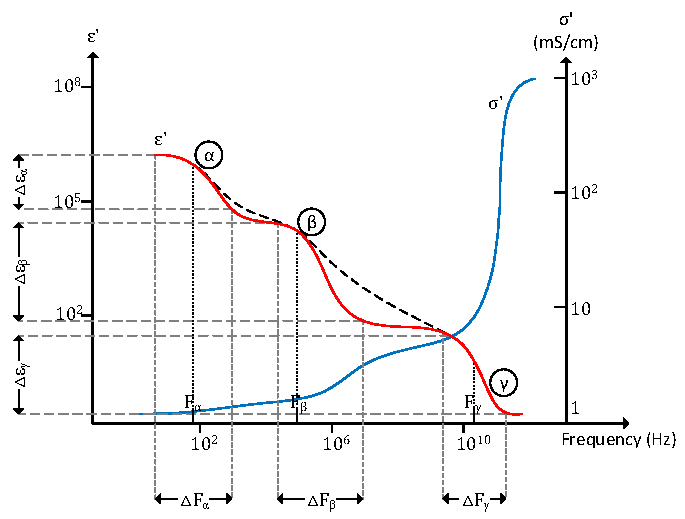
\includegraphics[width=0.8\textwidth,keepaspectratio, trim={0cm 1cm 0cm 0cm},clip]{figure3}    
	\caption[Alpha, Bet y Gama dispersion]{Representation of a cell with its electric characteristics. Internal cytoplasm characteristic permittivity $\epsilon_{cp}$ and conductivity $\rho_{cp}$. Extracellular fluid permittivity $\epsilon_m$ and conductivity $\rho_m$). Membrane permittivity described as ($\epsilon_{MBR}$) and conductivity ($\rho_{MBR}$).}
	\label{fig:ABG dispersion}
\end{figure}

In addition, the $\beta$ dispersion region provides supplementary information about the cell. Lvovich \cite{lvovich2012impedance} has divided this area into three subregions depending on the interaction of the electrical current with the cell. The $\beta_1$ relaxation is due to the capacitive membrane $C_m$, occurring in the low \si{\kilo\hertz} range. When the frequency is increased between \si{\kilo\hertz} and low \si{\mega\hertz} range the internal cytoplasm of the cell can produce a $\beta_3$ dispersion because of a change from resistive to capacitive conduction. However, this capacitive component is often disregarded simplifying the model into just a resistive element $R_i$. Ultimately, $\beta_2$ happens in the range of low \si{\mega\hertz} when the electrical charge movement through the cell shifts to a capacitive conduction.

This research document is centred in the $\beta$ dispersion region between \SIrange[scientific-notation = engineering]{100}{1000000}{\hertz}. The impedance plethysmography device designed described in chapter \ref{chapter design} is capable to operate within this bandwidth. 

The ideal electrical model of the cell shown in figure \ref{fig:cell models} is a very close approximation that allows predicting bioelectrical impedance behaviour for dilute cell suspension. However, tissue is more complex than this having extra components to be analysed. For instance, tissue like muscle exhibits extreme anisotropy (conductivity is not the same when measured in different directions) \cite{lvovich2012impedance,dean2008electrical,foster1995dielectric}. Therefore, the position where electrodes are placed influences in the impedance of the readings. Also the change of volume of the blood vessels during the heart’s systole and diastole also changes impedance magnitude readings which is the principle used by impedance plethysmography. 

Another example of this is in the myocardial muscle studied in pigs where two superimposed depressions were observed in-between \SIrange[scientific-notation = engineering]{10}{1000000}{\hertz} ~\cite{casas1999vivo}. Different resistivity values have been obtained when measuring bioelectrical impedance during the cardiac cycle longitudinally and transversally \cite{steendijk1993four}. \mynote{Maybe this paragraph is not requires as might refer to death cells rather than plethysmography}

%********************************** %First Section  **************************************
\section{Impedance plethysmography principle} %Section - 1.1                                                                                                                                                                                                 
\label{section impedance 1}
Referred as impedance plethysmography (iPG) involves the measurement of the change of impedance due to change of blood flow. For instance, when heart’s systole increases blood flow, the volume of a limb rises due to the inflow of blood (swelling)~\cite{martinsen2011bioimpedance}. Consequently, there are changes of impedance correlated to the changes of volume and flow in a limb. Some medical application might require the use of occlusion cuffs to analyse venous filling. There are several medical applications for this kind of technique such as heart stroke volume (SV) measurement, cardiac output (CO), thoracic respiratory volume, oedema and detection of deep vein thrombosis (DVT)~\cite{holohan1996plethysmography}.

As previously described in section \ref{section literature 3.5}, iPG is the measurement of volume changes through the equivalent bioelectrical impedance of a part of the human body~\cite{corciova2011peripheral}. In this document is presented the measurements from an in-vivo studio of the plethysmographic changes in a segment of the left forearm. As it can be deduced, one would assume that this segment of the upper limb could be modelled as a cylinder within a cylinder. Where the inner cylinder represents a blood vessel and the outermost is the surrounding tissue. 

For mathematical analysis, a single cylinder will be initially studied and then the double cylinder model. An ideal circular solid model can be applied where the cross-sectional area might have a circular or elliptical form. Hence, measurement of electrical impedance might depend on its geometry. The following equation illustrates the segment’s geometry effects either conductance ($G$) or resistance ($R$). However, this document will use the resistance equivalent during the mathematical explanation.

\begin{align}
\label{eq:resistivity}
R=\sigma\frac{L}{A}
\end{align}


where $\rho$ is the tissue’s conductivity, $A$ the cross sectional area of the cylinder and $L$ its length. From conductance equation can be deducted that if length increases conductance will decrease. Opposite, if the volume of the cross section $A$ increases then conductivity will increase. A representation of this cylinder can be seen in \ref{fig:cylinder model}. Hence, it is possible to find the volume as function of its resistance can be described with the following equation.

\begin{align}
\label{eq:volume (R)}
v=G \rho L^2 = R\sigma A^2 = \frac{1}{R} \frac{L^2}{\sigma}
\end{align}

\begin{figure}[!htpb]
	\centering
	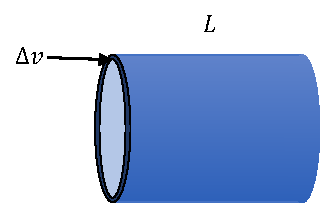
\includegraphics[width=5.5cm,keepaspectratio]{figure4}    
	\caption[Cylinder model for impedance calculation]{Cylinder model of length L and parallel volume increment}
	\label{fig:cylinder model}
\end{figure}
 

It must be noticed from the previous equation that if $L$ is constant then volume $v$ is directly proportional to the conductance $G$. However, if the presumption is that the area $A$ is constant then volume $v$ is directly proportional to resistance $R$. In the case of human blood vessels, it is expected that swelling occurs transversely. In this case, a rise of volume $\Delta v$  is better represented as conductance increase in a parallel model~\cite{martinsen2011bioimpedance}. Hence, when a variation of volume $\Delta v$ occurs a change of impedance $\Delta G$ might also be present. As a result, both entities can be expressed as a relation between two parameters as shown in the equation below.

 \mynote{Probably I should use the description I made from the Nyober equation}

\begin{align}
	\label{eq:volume (deltav)}
	\frac{\Delta G}{G} = \frac{\Delta v}{v} \qquad\text{or}\qquad \frac{\Delta G}{G} = \frac{\sigma}{L^2} \qquad\text{or}\qquad \Delta v = \Delta G \rho L^2
\end{align}


The same equation can be also represented as function of a change of resistivity $\Delta R$. In this case the equation changes to \ref{eq:volume (deltaR)}. It must be kept in mind that the minus sign represents that a resistance increase corresponds a volume decrease \cite{martinsen2011bioimpedance}. 
 
\begin{align}
	\label{eq:volume (deltaR)}
	 \Delta v \cong \Delta R \rho \bigg( \frac{L}{R} \bigg)^2 \qquad (\Delta R \ll R)
\end{align}

Nevertheless, a human body segment could be sculpted as two-compartment cylinder model where length $L$ is constant and the two cylinders are physically in parallel (see figure \ref{fig:two cylinder modell}). Supposing that the volume of the inner cylinder is equivalent to $\Delta v + v_A$ and $v_t$ is the constant outer cylinder volume. Then, the following equation represents the change in conductivity when both tubes swell $(\Delta v > 0)$. From that equation can be deduced that the problem of high sensitivity plethysmography depends on selectively measuring the immittance in a selected volume~\cite{martinsen2011bioimpedance}.

\begin{figure}[!htpb]
	\centering
	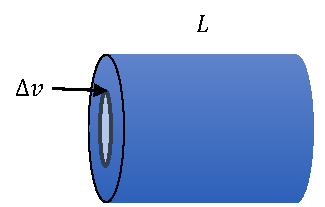
\includegraphics[width=5.5cm,keepaspectratio]{figure5}    
	\caption[Two compartment cylinder model]{Two compartment cylinder model of length L and parallel volume increment}
	\label{fig:two cylinder modell}
\end{figure}

In this case, the conductivities and cross section areas from surrounding tissue ($\sigma_t$) with area $A_t$ and tissue ($\sigma_b$) with area $A_b$ will also contribute towards the total conductance $G$ of the segment. Consequently, considering constant geometry, the conductance of these two cylinders could be expressed as the following equation.

\begin{align}
G = (\sigma_b A_b + \sigma_t A_t) \frac{1}{L}
\end{align}

However, the previous equation does not represent plethysmography because area change has not been assumed when swelling occurs. But as Grimmes et al.~\cite{martinsen2011bioimpedance} describes the previous equation 'relates to flow system with a varying conductivity of the passing liquid, and flow with time is volume'.

But a segment of human body limb is a dynamic system where the cross sectional area changes with the pulsatile movement of the arteries.  For instance, when a blood bolus volume goes through an artery there is a temporary increase of local volume during heart systole (see figure \ref{fig:cylinder bolus}). There are different blood flows occurring during a heart cycle in the inner cylinder of the selected segment that is the blood vessel. First, during inflow phase blood vessel is filled, then during outflow phase, the diastole heart cycle transports blood further down but at the same time is returning through the venous system.


\begin{figure}[!htpb]
	\centering
	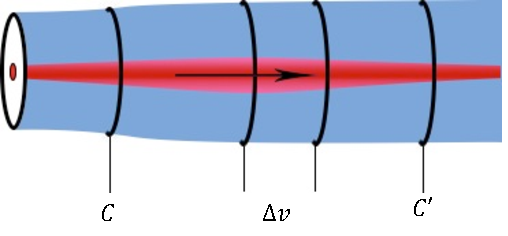
\includegraphics[width=7cm,keepaspectratio]{figure6}    
	\caption[Four electrodes placement for iPG]{Four electrodes system with the effect of a bolus of blood passing through a selected segment}
	\label{fig:cylinder bolus}
\end{figure}

For this reason tetrapolar method or four electrodes measurement are desirable as displayed in figure \ref{fig:cylinder bolus}. Some of the reasons exposed are that is easier to confine the measured tissue volume to the area of the volume increase. Also, the sensitivity will depend on the bolus length in relation to the measured distance between electrodes may also increase sensitivity~\cite{porter1985measurement}.


%********************************** %Second Section  *************************************
\subsection{Blood contribution to impedance} %Section - 3.2.1
As it has been described impedance plethysmography relies on the change of volume caused by blood vessels filling up all along the cardiac cycle. Nonetheless, blood is highly conductive and influences the amplitude of the waveform. However, there are also particular properties that might modify its intrinsic signal. In one of the earliest research about the conductivity of blood, Sigman et al.~\cite{sigman1937effect} \mynote{Check if I can find a more updated version of this} demonstrated that resistivity of blood depends on its flow.  It was found that when blood velocity decreased from \SIrange{10}{40}{\centi\meter\per\second} its resistivity fell roughly \SI{7}{\percent}. Blood can be simplified as a suspension of particles (erythrocytes or RDC) with a high resistivity floating in a conductive medium (plasma). The rest of blood’s cells do not represent a great component in the change of impedance because of its small size in comparison with the erythrocytes (see table \ref{table:cell}). In fact, the Sigman effect is not presented in either plasma or electrolytes~\cite{tremper1990principles}.  

It has also been proved that blood is electrically anisotropic because of the orientation of the RBC’s \cite{Visser1992Electric}. Moreover, geometry and orientation also affect the reading of resistivity. Which also means that direction of measurement also affects the readings. 
 

%********************************** % Third Section  *************************************
\section{Electrode conflict}  %Section - 3.2 
\label{section impedance 2}
Electrodes play a key feature in a bioelectrical impedance system. The right electrode geometry, distance and material may influence in the readings from a biological sample. Consequently, it is needed to use electrodes that have minor impedance compared to the one from the subject under test. Currently, most common materials used in bioelectrical impedance are platinum (\textit{Pt}), gold (\textit{Au}) or stainless steel. Other independent variables such temperature, ionic tissue contents and protein adhesion influence in the change of electrode impedance~\cite{ivorra2003bioimpedance,martinsen2011bioimpedance}. The geometry of the electrode also affects its resistance ($R$) as explain by ohm’s law in equation \ref{eq:resist}.

\begin{align}
	\label{eq:resist}
	R = \rho \frac{L}{A}
\end{align}

where $\rho$ is the electrical resistivity of the material, $A$ is the area of the electrode and $L$ its longitude or thickness. As it can be noticed, the resistance ($R$) reduces when the area ($A$) of the electrode increases. However, the total resistance ($R$) is directly proportional to the electrodes length. 

When an electrode adheres to the skin, and electrical current passes through, a physical effect takes place. First, there is an electrical charge change from electronic to ionic conduction because inside the body the latter is only possible. Second, at the electrode–tissue boundary an electrochemical reaction follows, called electrolysis. This effect creates a “double layer capacitance (DLC)” (see figure \ref{fig:DLC}) that as its name indicates, adds a capacitive effect to boundary \cite{lvovich2012impedance}.  Consequently, applying an AC waveform inverts the electrode’s polarity during each cycle minimising this capacitive effect. However, this is a frequency dependent development, which means that at low frequencies can be quite notorious \cite{bertemes2002tissue}.  

\begin{figure}[!htpb]
	\centering
	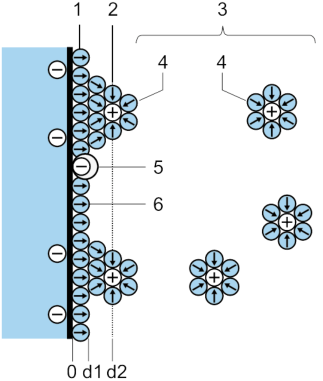
\includegraphics[width=5.5cm,keepaspectratio]{figure7}    
	\caption[Dual layer representation on an elecgtrode]{Schematic representation of a double layer on an electrode (BMD) model. 1. Inner Helmholtz plane, (IHP), 2. Outer Helmholtz plane (OHP), 3. Diffuse layer, 4. Solvated ions (cations) 5. Specifically adsorbed ions (redox ion, which contributes to the pse)}
	\label{fig:DLC}
\end{figure}

\mynote{I have to reference this section. I think is from Martinesen}

An electric circuit model can represent the electric–tissue interface; this simplified electric representation is shown in figure \ref{fig:e-t circuit}. In more detail, this model is characterised by a charge transfer resistance ($R_{CT}$) in parallel with interface’s impedance ($Z_{CPE}$) in series with the tissue impedance ($Z_t$).  Some authors have defined the interface’s impedance as either a constant phase angle impedance ($Z_{CPA}$)~\cite{franks2005impedance} or constant phase element ($C_{PE}$) \cite{barsoukov2005impedance,mcadams2006characterization}. 

The value of $Z_{ZPA}$ can be calculated from the following empirical equation \ref{eq:zcpa} given by McAdams~\cite{mcadams1995linear}.

\begin{align}
\label{eq:zcpa}
Z_{CPA} = K(j\omega)^{-\beta}
\end{align}

where $K$ is a measure of the magnitude of $Z_{CPA}$, $\beta$ is a constant ($0 \leq \beta \leq 1$) representing inhomogeneities in the surface (typically \num{0.8} for many biomedical electrode systems) and $\omega = 2\pi f$. When $\beta = 1$, $Z_{CPE}$ is equivalent a purely capacitive impedance element \cite{franks2005impedance,mcadams1995linear,mcadams2006characterization}.


\begin{figure}[!htpb]
	\centering
	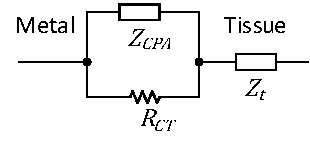
\includegraphics[width=5.2cm,keepaspectratio]{figure8}    
	\caption[Equivalent circuit electrode–tissue interface]{Equivalent circuit electrode–tissue interface (Adapted from Franks~\cite{franks2005impedance})}
	\label{fig:e-t circuit}
\end{figure}


%********************************** %Nomenclatures in chapter  **************************************
\nomenclature[z-EM]{EM}{Electromagnetic}
\nomenclature[z-EIS]{EIS}{Electrical impedance spectroscopy}
\nomenclature[z-BLM]{BLM}{Bilayer lipid membrane}
\nomenclature[z-DLC]{DLC}{Dual layer capacitance}